\documentclass[11pt,a4paper]{report}
\usepackage[left=3cm,right=3cm,top=3cm,bottom=3cm]{geometry}
\usepackage[utf8]{inputenc}
\usepackage[francais]{babel}
\usepackage[T1]{fontenc}
\usepackage{graphicx}
\usepackage{blindtext}
\usepackage{listings}
\usepackage{amsmath}
\usepackage{amssymb}

\makeatletter
\renewcommand{\@chapapp}{Exercice}
\makeatother

%\setlength{\parindent}{0.7cm}
\setlength{\parskip}{\baselineskip}

\begin{document}

\begin{titlepage}

\centering

\includegraphics[scale=0.4]{SU.png}\par\vspace{1cm}
\vspace{1cm}
{\scshape\bfseries ARA\par}
\vspace{1.5cm}
{\huge\bfseries Projet Peersim\par}
\vspace{2cm}
{\Large\itshape Robin Blottiere-Mayo\par
	Pierre Oumeddour\par}
\vfill
{\Large Professeur : Jonathan Lejeune}
\vfill

% Bottom of the page
{\large \today\par}
\end{titlepage}

%\title{ARA}
%\title{Projet Peersim}
%\author{Robin Blottiere-Mayo\\
%	Pierre Oumeddour\\
%	Professeur : Jonathan Lejeune}
%\date{\today}

%\maketitle

\pagenumbering{arabic}

\chapter{}

\section{Question 1 :}

L'algorithme de verrouillage utilisé dans la classe Application est un algorithme dérivé de celui de Naimi-Tréhel utilisant la notion de jeton.
%\linespread{0.5}

Ainsi tous les sites se partagent le même jeton et seul le site possédant le jeton peut entrer en section critique. Dans la classe Application, les constantes initial\_owner et nil servent à discriminer le site possédant le jeton des autres.
%\linespread{1.7}

Chaque noeud maintient sa propre liste de noeuds en attente de section critique (variable next) et son compteur global de sections critiques (variable global\_counter). Il possède également l'adresse du noeud dont il pense qu'il possède le jeton (variable last) ainsi que le nombre de sections critiques qu'il a lui-même effectuées (variable nb\_cs). Si un noeud veut une section critique, il envoie une demande pour avoir le jeton puis il se met en attente.
%\linespread{0.5}

Quand un noeud sort de section critique, il envoie le jeton au dernier noeud de la liste des noeuds demandant la section critique avec les informations qu'il possède du nombre de sections critiques réalisées et des noeuds en attente de section critique.
%\linespread{0.5}

Lorsqu'un noeud reçoit le jeton, il met à jour son compteur de sections critiques avec la valeur envoyée par le dernier noeud ayant été en section critique. Il compare également sa liste de noeuds en attente avec celle qu'il a reçue. Si des noeuds se trouvent dans les deux listes mais pas dans le même ordre, l'ordre envoyé par le dernier noeud en section critique est maintenu. Si des demandes sont absentes de la liste reçue, elles sont ajoutées en fin de liste.


\section{Question 2 :}

On considère trois états du jeton :
\begin{enumerate}
	\item Un noeud possède le jeton mais ne s’en sert pas (état tranquille).
	\item Un noeud possède le jeton et est en section critique (état utilisé).
	\item Le jeton est en transit (état enTransit).
\end{enumerate}

tranquille $\rightarrow$ utilisé : la section critique est demandée et personne ne requiert le jeton.\\
tranquille $\rightarrow$ enTransit : un noeud requiert le jeton.\\
utilisé $\rightarrow$ tranquille : la section critique se termine.\\
utilisé $\rightarrow$ enTransit : releaseCS(timeout) \& !next.isEmpty()\\
enTransit $\rightarrow$ utilisé : receive\_token()\\

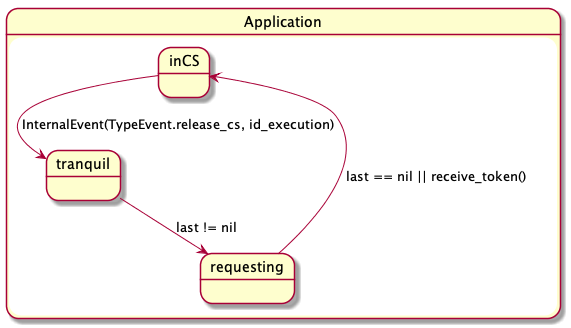
\includegraphics[scale=0.3]{../Diagrammes/exercice_1-question_2.png}


\section{Question 3 :}

$\alpha$ étant le temps moyen qu'un processus passe en section critique et $\beta$ le temps passé entre les sections critiques.

Le ratio $\rho$ = $\alpha$ / $\beta$ représente la charge du réseau.

Plus ce ratio est élevé plus le réseau est ralenti.

\section{Question 4 :}

\section{Question 5 :}

Le fait que le temps de transmission moyen soit supérieur au temps moyen passé en section critique augmente la charge du réseau. Le temps de transport augmentant, le temps ou le jeton est possédé par un noeud est plus faible.

Cela ne change pas fondamentalement les résultats en dehors de rendre le système plus lent et de diminuer le nombre de section critique pour un temps d'exécution égale.

Dans le détail, on voit que les premiers instants du fonctionnement du système le noeud ayant le jeton peut exécuter plusieurs fois sa section critique avant de recevoir une requête et que la file des noeuds demandant l'accès à la section critique mettra plus de temps à se remplir. Cependant après que tous les noeuds aient exécuté au moins une fois leur section critique, le temps passé en section critique et le temps de transmission du message s'additionnant rendront la suite de l'exécution semblable à ce qu'elle aurait été avec un temps de transmission moyen plus faible que le temps passé en section critique.


\chapter{}


\chapter{}


\end{document}
